\section{File structure description with explanations of functionality of each
	part}\label{FileStructureDescriptionWithExplanationsOfFunctionalityOfEachPart}

This section outlines the file structure of UxAS with descriptions and
explanations of each part. Figure \ref{fig:UxASAndDependentProjects.png} shows the
UxAS folder and the folders housing its dependent projects. It is
recommended that the OpenAMASE, LmcpGen, and OpenUxAS projects are
placed in the same directory. The OpenAMASE project is used to run
simulations with simulated aircraft. The LmcpGen project is used to
generate LMCP messages.

\begin{marginfigure}[150pt]
	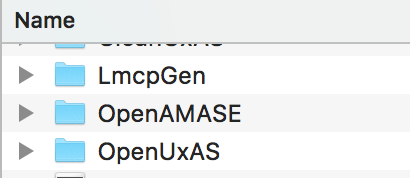
\includegraphics[width=1.3\linewidth]{\FiguresPath//UxasAndDependentProjects.png}
	\caption{Open UxAS Folder}
	\label{fig:UxASAndDependentProjects.png}
\end{marginfigure}

Within OpenUxAS there is a series of folders. These folders include 3rd,
doc, examples, mdms, resources, src, and tests. These folders can be
seen in figure \ref{fig:OpenUxASFolderContents.png}. The 3rd folder contains
UxAS's dependent libraries. The doc folder contains UxAS documentation.
The examples folder holds a series of configurations that are necessary
to execute a simulation with OpenUxAS and OpenAMASE. The MDMs folder
contains Message Data Modules that are used by LMCP to define custom
sets of messages for each target system. The resources folder contains a
series of scripts that can be used to analyze a simulation. The src
folder contains the source code for OpenUxAS. The tests folder contains
the unit tests.


\begin{marginfigure}[150pt]
	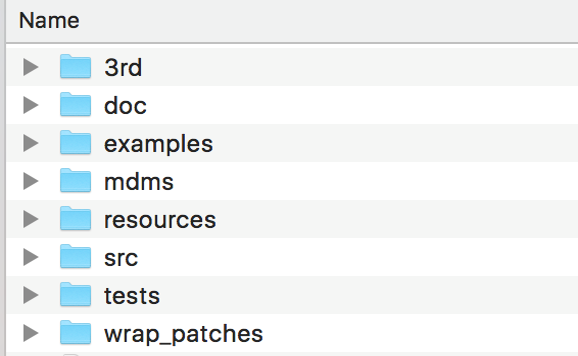
\includegraphics[width=1.3\linewidth]{\FiguresPath//OpenUxASFolder.png}
	\caption{Open UxAS Folder Contents}
	\label{fig:OpenUxASFolderContents.png}
\end{marginfigure}

The contents of the doc folder can be seen in figure \ref{fig:DocFolder.png}.
This folder contains additional folders named doxygen, LMCP, and
reference. The doxygen folder holds the files required to run doxygen
and perform code inspection with the doxygen output. The LMCP folder
contains files that describe the Message Data Modules. The reference
folder contains UxAS flow charts, sequence diagrams, and the UxAS user
manual.

\begin{marginfigure}[150pt]
	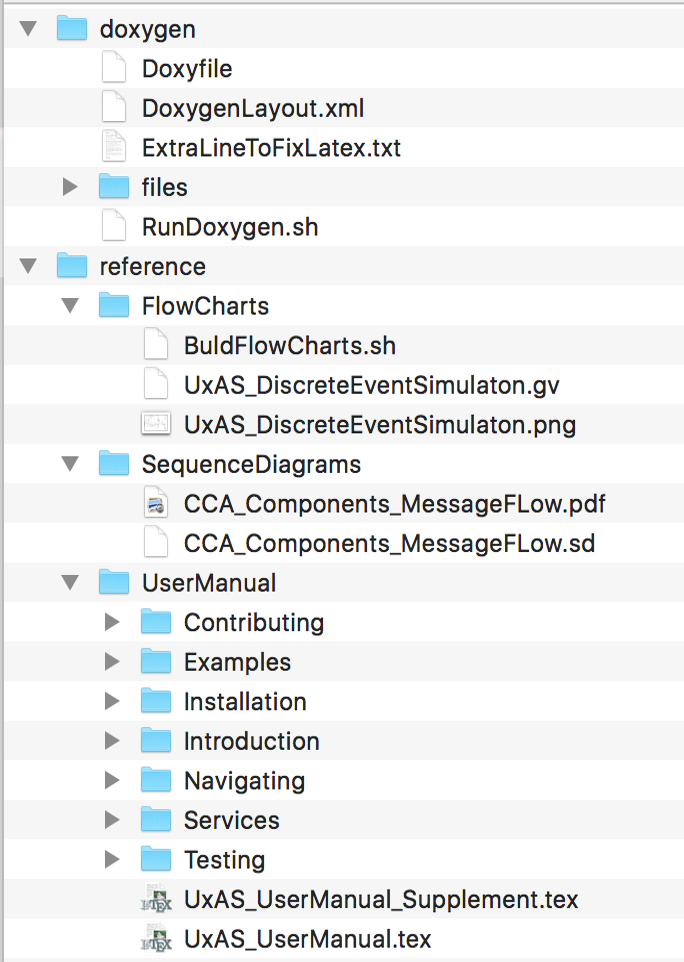
\includegraphics[width=1.3\linewidth]{\FiguresPath//DocFolder.png}
	\caption{Open UxAS Documentation Folder}
	\label{fig:DocFolder.png}
\end{marginfigure}

The examples folder contains folders that contain configuration files
required to execute a UxAS simulation. This folder can be seen in figure
\ref{fig:ExamplesFolder.png}. Most of the simulations cannot be executed without
OpenAMASE.

\begin{marginfigure}[150pt]
	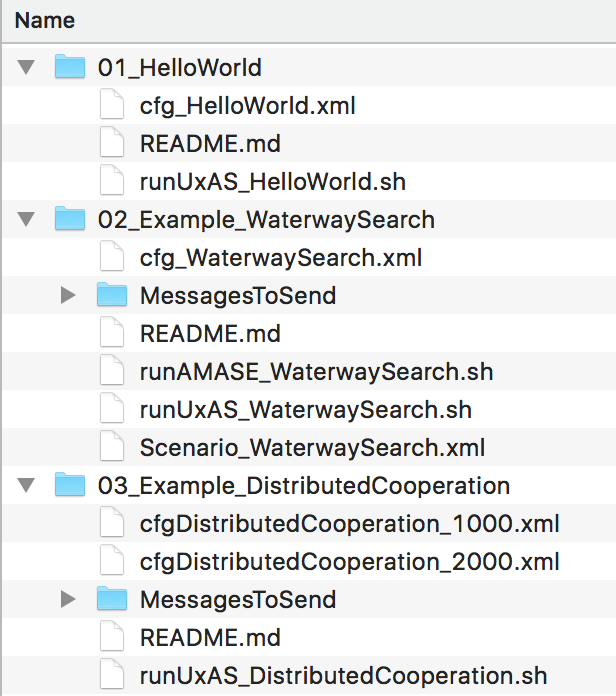
\includegraphics[width=1.3\linewidth]{\FiguresPath//ExamplesFolder.png}
	\caption{Open UxAS Examples Folder}
	\label{fig:ExamplesFolder.png}
\end{marginfigure}

The mdms folder contains the message data modules. This folder can be
seen in figure \ref{fig:MdmsFolder.png}. These configuration files are used by
LMCP to define custom sets of messages for each target system.

\begin{marginfigure}[150pt]
	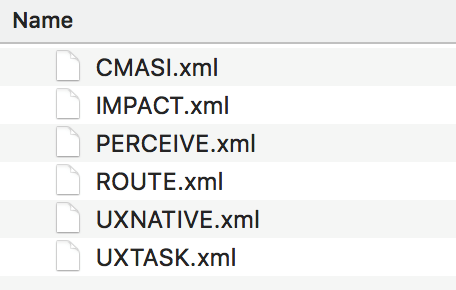
\includegraphics[width=1.3\linewidth]{\FiguresPath//MdmsFolder.png}
	\caption{Open UxAS Message Data Models Folder}
	\label{fig:MdmsFolder.png}
\end{marginfigure}

The resources folder contains a series of scripts that can be used to
analyze a simulation. The resources folder can be seen in figure
\ref{fig:ResourcesFolder.png}.

\begin{marginfigure}[150pt]
	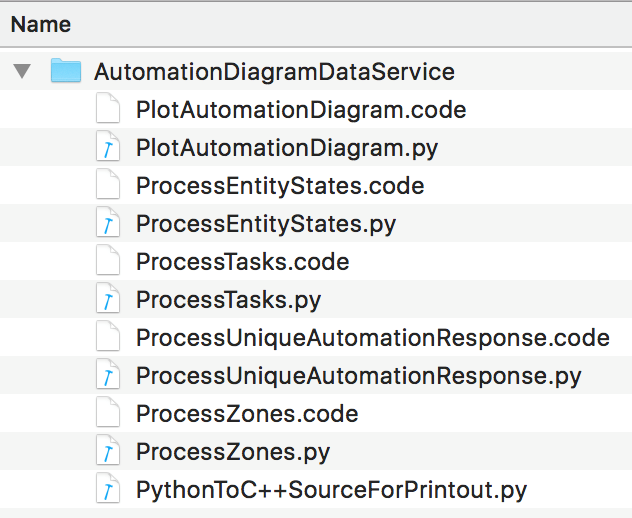
\includegraphics[width=1.3\linewidth]{\FiguresPath//ResourcesFolder.png}
	\caption{Open UxAS Resources Folder}
	\label{fig:ResourcesFolder.png}
\end{marginfigure}

The src folder contains the OpenUxAS source code. This includes all of
the header and implementation files. The contents of this folder can be
seen in figure \ref{fig:SrcFolder.png}.

\begin{marginfigure}[150pt]
	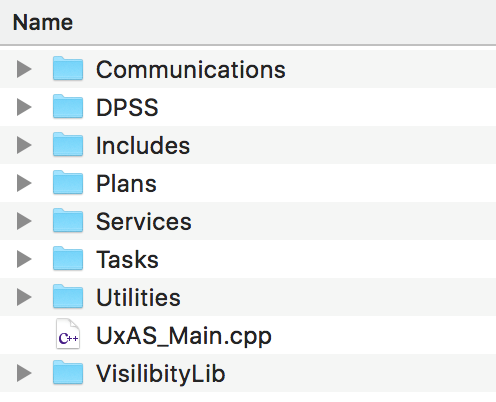
\includegraphics[width=1.3\linewidth]{\FiguresPath//SrcFolder.png}
	\caption{Open UxAS Source Folder}
	\label{fig:SrcFolder.png}
\end{marginfigure}

The test folder contains all the unit tests that can be run to assess
the messages that UxAS sends. This folder can be seen in figure
\ref{fig:TestFolder.png}.

\begin{marginfigure}[150pt]
	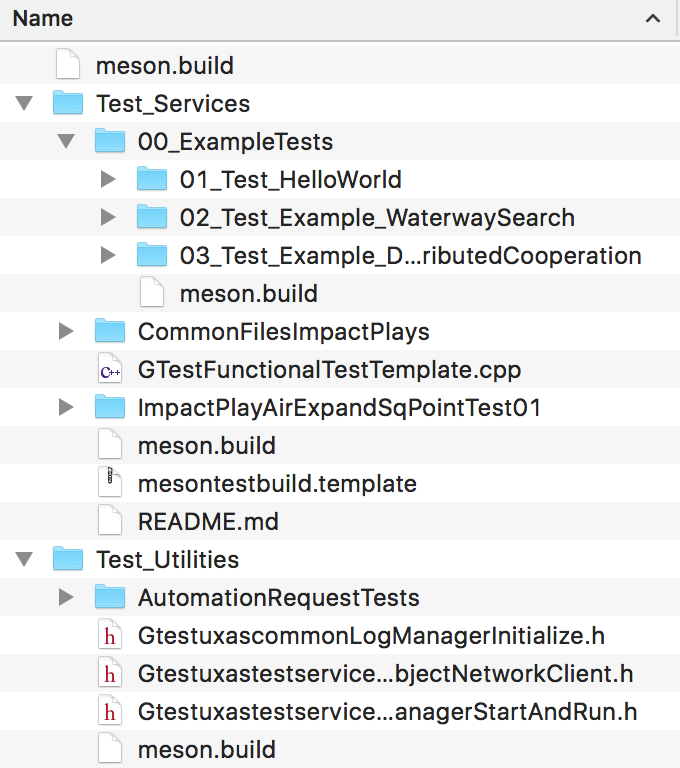
\includegraphics[width=1.3\linewidth]{\FiguresPath//TestsFolder.png}
	\caption{Open UxAS Test Folder}
	\label{fig:TestFolder.png}
\end{marginfigure}

\section{Architecture and Messaging}\label{ArchitectureAndMessaging}
